\documentclass[12pt]{report}
\RequirePackage{palatino}
\RequirePackage{verbatim}
\RequirePackage{amsmath,amsfonts,amsthm,amssymb,multirow,xcolor}
\RequirePackage{geometry}
\RequirePackage{graphicx}
\RequirePackage[useregional]{datetime2}
\RequirePackage{hyperref}
\graphicspath{ {images/} }
%===================================================
\renewcommand{\maketitle}{
\hrule height 1pt
\begin{center}
{\bf \large Meeting Notes}\\[2mm]
THEORY407, Fall 2022\\[2mm]
\end{center}
\hrule height 1pt
}
\graphicspath{ {./images/} }
%===================================================
\NewDocumentCommand{\datesec}{o m m}{%
    \renewcommand\thesection{\DTMdate{#2}}
    \IfNoValueTF{#1}
        {\section{#3}}
        {\section[#1]{#3}}
}
%===================================================
\geometry{left=1in,right=1in,top=1in,bottom=1in}

\begin{document}
\maketitle
\tableofcontents
\section*{\datesec{2022-9-23}{}}
\paragraph*{\href{https://www.humdrum.org/guide/ch01/}{Humdrum Ch.1}}

It seems like a tool used for analyzing music similar to music21. With multiple 
funtionalities, Humdrum can be used for counting specific notes, showing certain
voice in a piece, and sometime even some specfic analysis on 
harmonic/tonal funtions. It is more like a library of tools on my idea of 
searching how similar two pieces are. We can conduct research with the same
approch, but with different methods. Starting with these simple metrics:
\begin{itemize}
    \item \textbf{Note Sequence}: How many notes are the same, how many are different?
        \begin{itemize}
            \item Might be useful for comparing two pieces in the same work, such as 
            \emph{Gymnopedie}. But will yield a very low score if the key changed.
        \end{itemize}
    \item \textbf{Note Sequence with Key}: How many notes are the same, given pieces 
    in different key but represented in a $\mathbb{Z}_7$ format.
    \begin{itemize}
        \item Can address some very basic isssues such as exact transposition,
        but not effective if the phrase changes. 
        \item Can use the technique mentioned in the proposal to
        solve the above problem. But what if the phrase was changed a lot?
    \end{itemize}
\end{itemize}
We then shall do the analysis with more and more complex methods such as counting
leading tones, and chords using current avaliable tools. In this way I believe we can come up with 
various ways to compare two pieces, but not being too impractical to do. The ultimate
goal is also simple: output a "similarity score" for two pieces.
\paragraph*{Will Read:}
\begin{itemize}
    \item Temperley, \emph{A Bayesian Approach to Key Finding}
    \item Lerdahl, \emph{Tonal Pitch Space} \textbf{Chapters *}
    \item Tymoczko, \emph{Geometry of Musical Chords} \textbf{Chapters *} 
\end{itemize}

\section*{\datesec{2022-11-4}{}}
\paragraph*{Test on modal music}
The Krumhansl-Schmuckler was tested on Bartok's \emph{14 Bagatelles Op.47 No.1}. The
algorithm regonized the right hand part as in E major/C\# minor, but ignored
the entire left hand in C Locrian/G Lydian. This is expected, since
the algorithm only outputs one key given all notes in the piece and 
it seems like notes in the left hand sums up to a less duration than
the right hand. So the KS algorithm put more weights in right hand than the
left. 
\\Link to a playable score:\url{https://musescore.com/user/4887176/scores/6403822}
\subparagraph*{Potential Solution}
We might do twice for the treble and bass clef seperately(limited to piano),
and then see if the two keys are the same. If they are, then we can say the
piece is in one key. 
\subparagraph*{Question}
How do we determine whether we should talk about keys seperately?

\paragraph*{Set-Class Similarity and Fourier Transform by Tymoczko}
Fourier transform assign two-dimensional vector whose components are:
\[V_{p,n}=(\cos(2\pi pn/12), \sin(2\pi pn/12))\]
Where for integer $n$ from $0$ to $6$ and $p$ in $\{0...11\}$ is the pitches
in a chord. Each fourier component is the sum of all such component:
\[n\text{th Fourier Component}=\sum_{p\in v}V_{p,n}\]
\begin{itemize}
    \item Voice leading and set-class similarity. Steps
    to find the minimal Euclidean voice leading between two n-note 
    multiset-classes $A$ and $B$:
        \begin{itemize}
            \item Choose a representative (prime form?) of $A$ calculate 
            the sum of its pitch classes.
            \item Find the $n$ (12/n semitones for each) 
            transpositions of $B$ with the same sum.
            \item For each of the transposition, calculate the $L_2$
            norm of $A$ and the vector. Do the same for inversions.
            \item Take the minimum of these $2n^2$ numbers and output the 
            result.
        \end{itemize}
    \item Fourier Magnitude
        \begin{itemize}
            \item In a set class space constructed by pitches of some 
            perfectly even $n$-note chord, $n\in\{1...6\}$. Note the $n$-note
            chord means the chord even seperate the $12$ tone equal 
            temperament pitches. 
            \item Given a $x$-note set-class space, the $n$th Fourier component of a chord will decrease 
            as pitches move away from the subset of pitches in $n$ notes 
            chord. Illustrated below:
            \begin{figure}[h]
                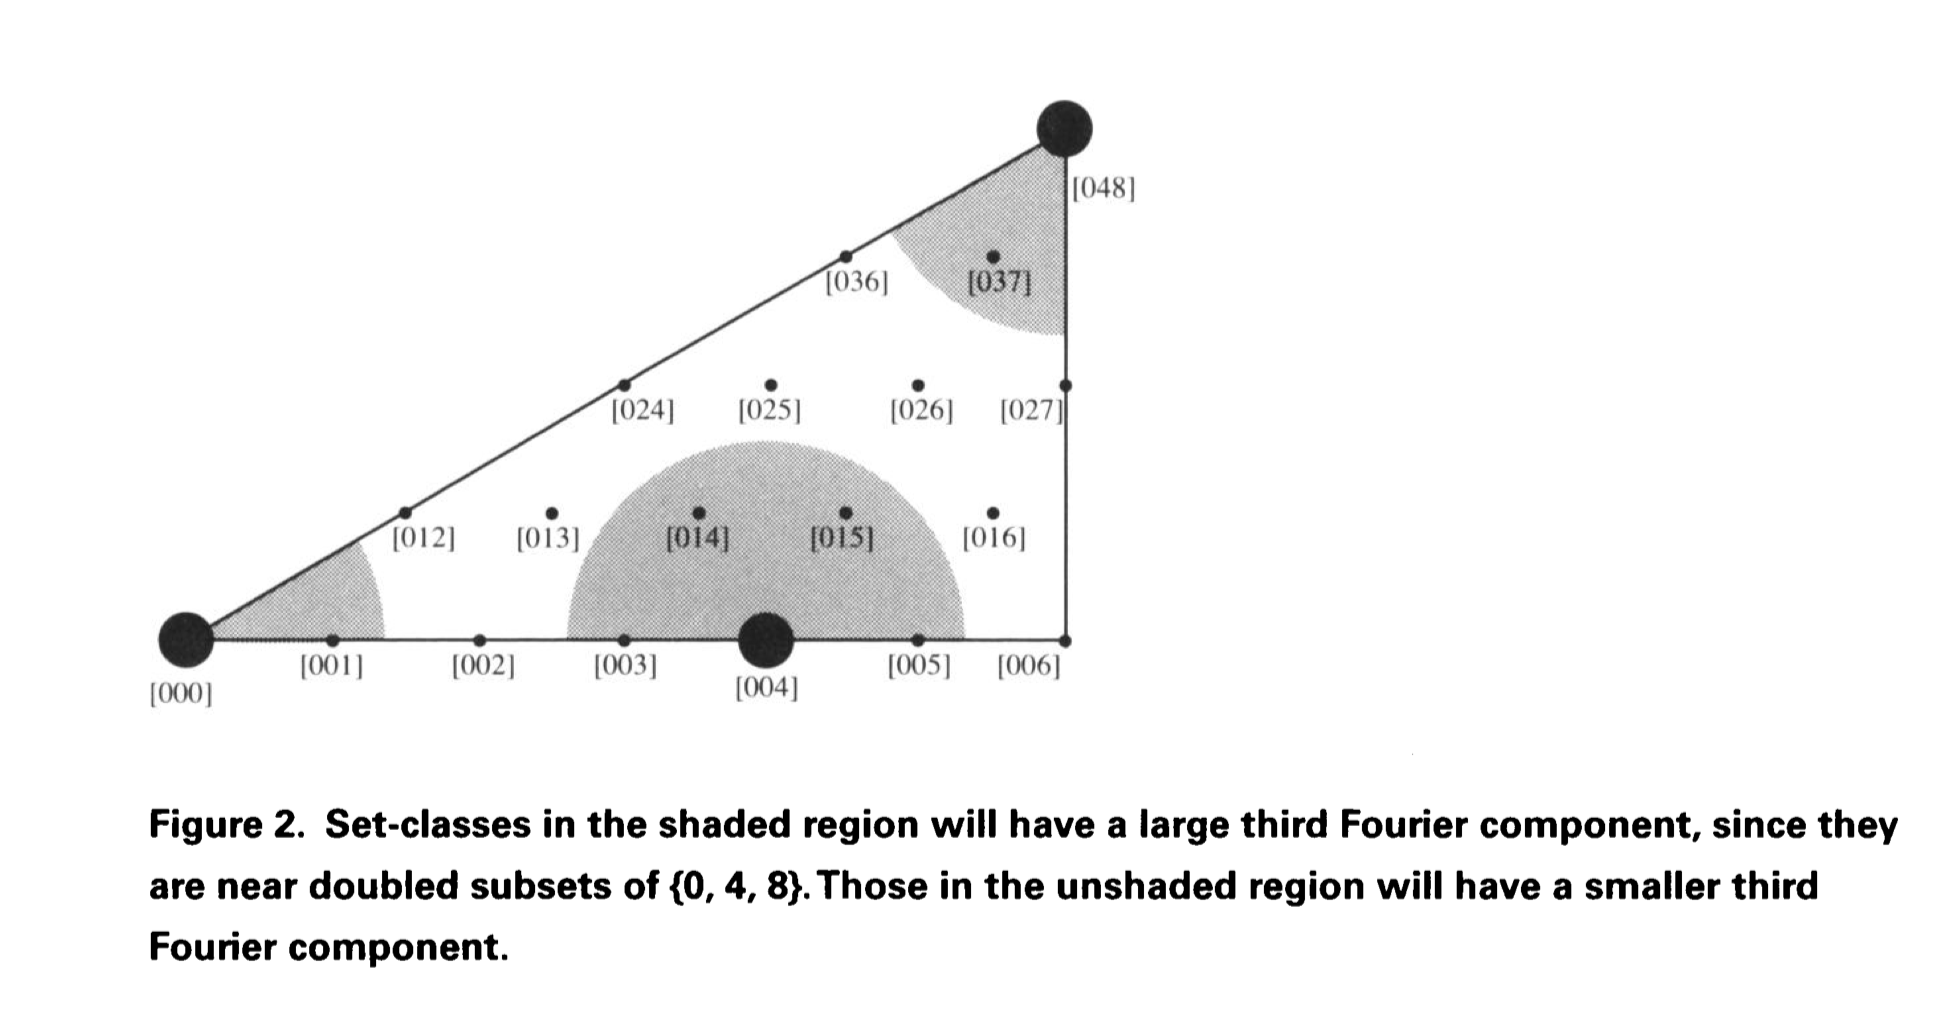
\includegraphics[scale=0.5]{Tymoczko_1.png}
            \end{figure}
            \item We can use a linear equation to estimate the $n$-th
            Fourier component of chord given the \emph{minimal voice leading
            } to the nearest doubled subset(VL). This means there is a 
            close relationship between FC and the minimal Euclidean distance 
            between two chords.
            \item 2 analysis procedure below:
            \begin{figure}[h]
                \centering
                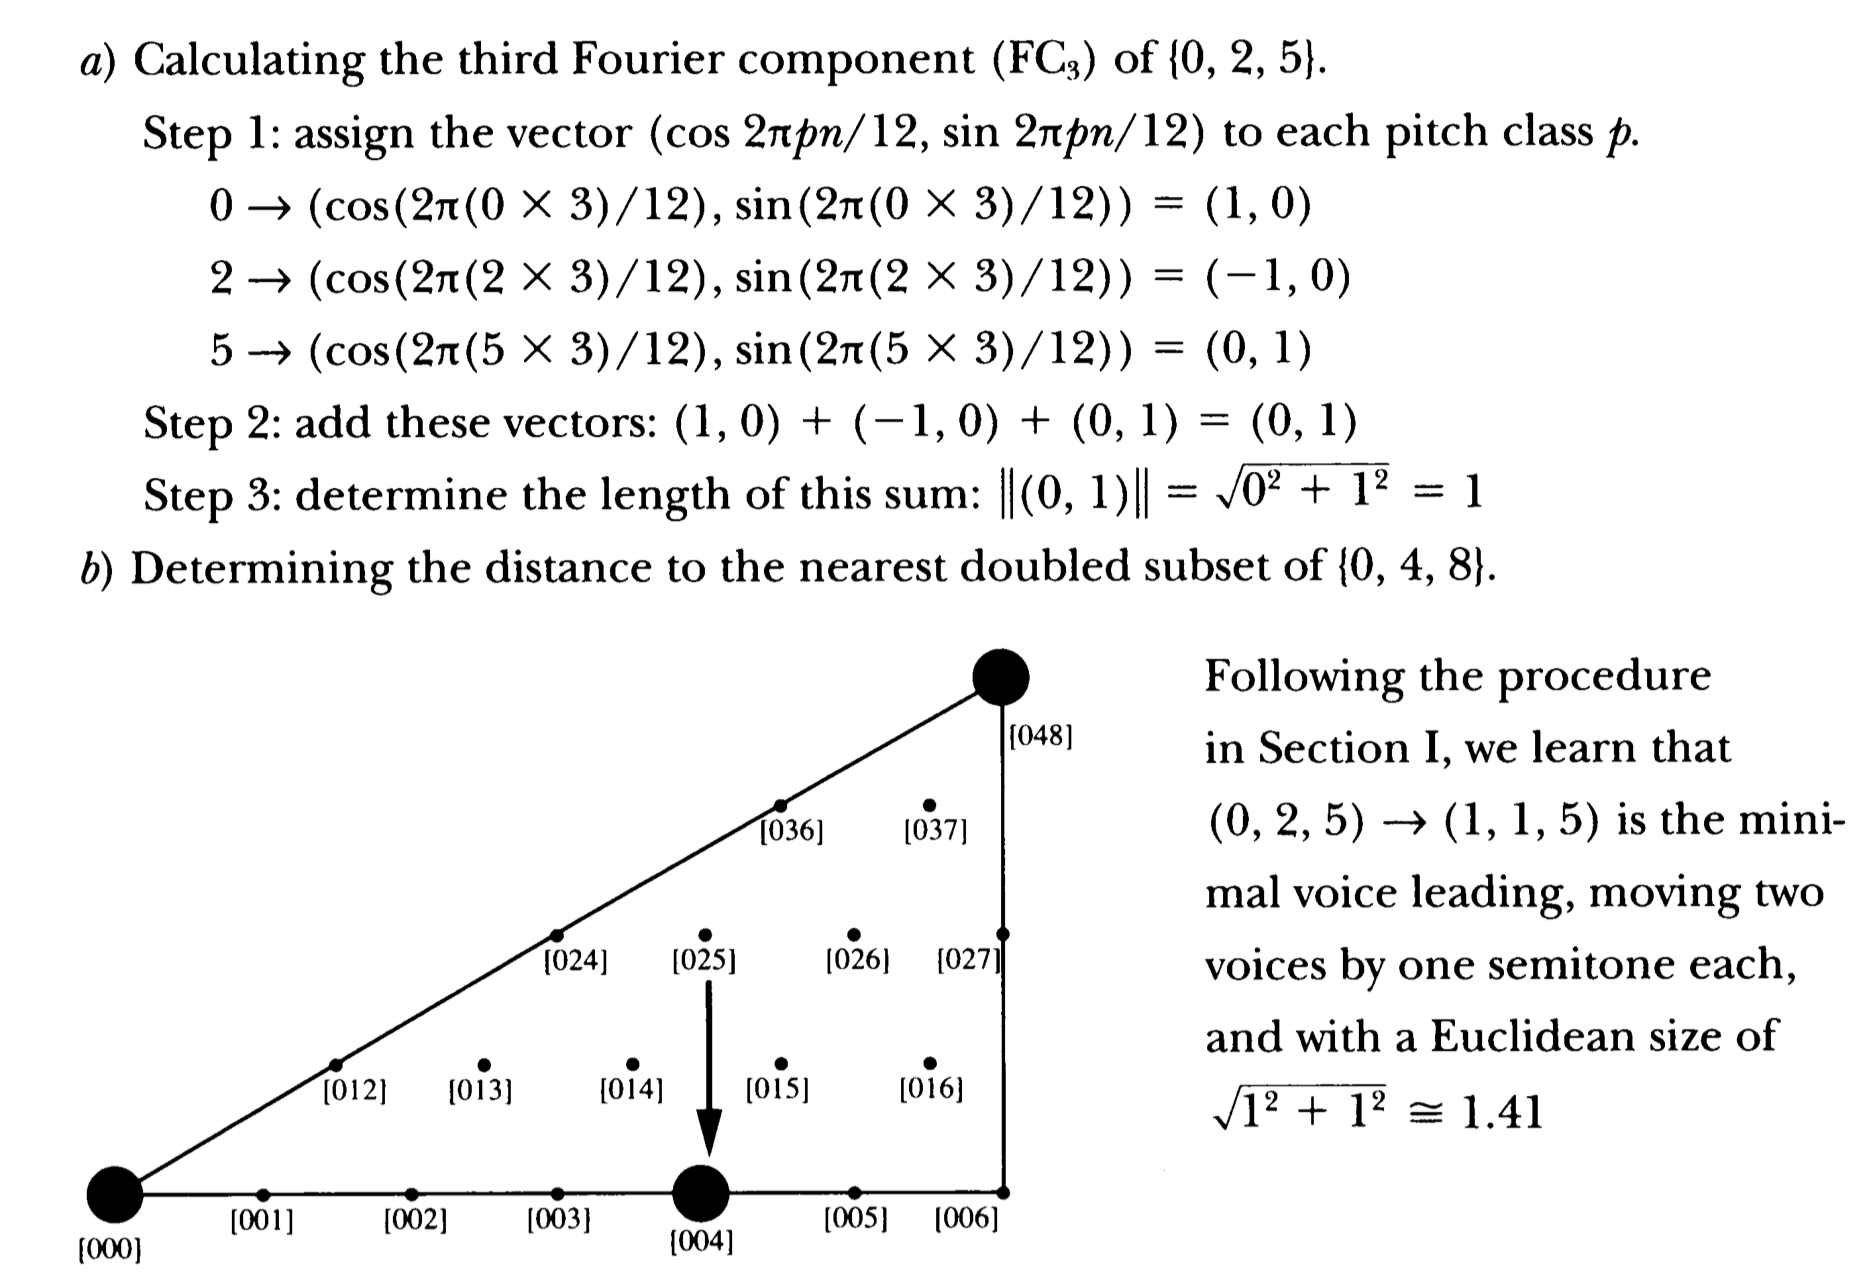
\includegraphics[scale=0.5]{Tymoczko_2.png}
            \end{figure}
            \item The analogy of minimal voice leading on 
            a pitch class circle is: as the Fourier Component increases
            (which is the sum of all vectors), the minal voice leading decreases.
            \item FC6 is the difference absolute value of difference between 
            the number of a chord's notes in one whole tone scale and the nuber 
            of its notes in the other ($[0,2,4,6,8,10],[1,3,5,7,9,11]$).
        \end{itemize}
\end{itemize}
\paragraph*{Reflectiond and Questions}
\begin{enumerate}
    \item Both Temperley and Tymoczko are trying to find the 
    similarity in terms of "fitness" to a certain pitch set class.
    In Temperley's case, it is the fitness to major and minor scale,
    while in Tymoczko's case, it is the fitness to a certainn evenly distributed
    $12/n$-notes chord. 
    \item What is the purpose of doing this? For Tymoczko, maybe it is
    demonstrating certian piece confirms such minimal voice leading motion?
    \\\url{http://dmitri.mycpanel.princeton.edu/ChordGeometries.html}
    \item So it seems like the notion of "motion"(no puns intended) here is
    important, how should we show such motion and make analysis upon it?
\end{enumerate}
\paragraph*{A proposed struture to show such motions}
This is only a speculative model to show such motions in terms of
intervals through time. Fix certain time untis and a pitch class space
($k$-euqal temperament) we can represent a piece of music as intervals
between notes in the same voice through time. For each voice,
if the piece alst for $m$ time units, there would be a 
1D array of size $m-1$ where the each entry of the array is the
interval between the pitches $n_i, n_{i+1}$ on time $i, i+1$. We 
can also counts the intervals between all voices on the same time
(Lewin's $\mathsf{IFUNC}$) and utilize his Fourier test for further
analysis. Given a proper time unit, we can also represent a "segment"
of notes by finding the closest "evenly distributed pitch class set"(Tymoczko's)
and then do analysis in terms of these summarized segments in correspondence
with the notion of "notes, phrase, section, passage".
\paragraph*{Questions}
\begin{enumerate}
    \item How do we determine a proper time unit?
    \item What kind of analysis shall we use for the horizontal interval vectors?
    \item This is most suitable for piano/counterpoint, what about other instruments?
\end{enumerate}
\paragraph*{Will Read:}
\begin{itemize}
    \item Tymoczko's Geometry of Chord Spaces
    \item Issacson's The Interval Angle
    \item Yust's Set Theory
\end{itemize}

\section*{\datesec{2022-11-27}{}}
\paragraph*{Yust's Set Theory}
Introduced Fourier componenets and phase spaces. 
\begin{itemize}
    \item \textbf{n Phase Space}: A circle evenly divided by $n$ interval(in the context of 12-equal temperament).
    \item \textbf{Fourier Component}: See summarization for Tymoczko's paper.
\end{itemize}
The process is similar to DFT, which can be seen as a matrix multiplication written as:
\[F_k=\frac{1}{n}\sum_{j=0}^{n-1}e^{-2\pi i\frac{jk}{n}}\]
Where $F_n$ is the $n$-th Fourier component, $k$ is the pitch class, and $n=12$. Or, more generally:
$\hat{f_k}=[[\mathsf{DFT}]]\cdot f_k$. Think of the process as matrix multiplication.
Different phase space reveals different properties of music. $Ph_5$ indicates 
the a set's affinity toward diatonic collection. Each $6$ phase space approximates:
\begin{enumerate}
    \item chromaticism
    \item quartal harmony?(not sure what this means)
    \item hexatonicity
    \item octatonicity
    \item diatonicity
    \item whole-tone quality.
\end{enumerate}
\emph{Scale Theory? Eveness? Might need more explanation.}
We can also use DFT to calculate the common tones of two sets. 
\[\frac{1}{12}\sum_{n=0}^{11}|f_n(A)||f_n(B)|cos(\phi_n(A)-\phi_n(B))\].Intuitively,
common tones will show harmonic closeness. Another aspect in the common tone analysis
is the "wormhole" effect. Which is simply apply analysis in two phase spaces.

\paragraph*{Questions}
\begin{itemize}
    \item What can I do for DFT in the interval space?
    \item Since DFT can be seen as a matrix operation, what does the eigen value of a DFT matrix show?
    \item Structure for my writing toward the end of calss?
\end{itemize}
\paragraph*{Will Read:}
Isaacson's The Interval Angle
\section*{Segmentation task}
Segmentation is a cognitive process that "selects structually significant 
intervallic relations" according to Hasty. The process itself involes with 
decisions based on multiple aspect/"domains" of music properties such as
dynamic, timbre, set class etc. There are two ways to do segmentation task using 
computers:
\begin{enumerate}
    \item \textbf{Bottom-up}: Start from the smallest unit of each domain and write 
    scripts for them. But difficulties occurs in defining herustics for each domain such 
    as searching for "strongest" set class in given phrase.
    \item \textbf{Machine Learning}: Build a machine learning model 
    that can learn from the data and make segmentation decisions. But it is
    difficult to find a proper training set and the model itself is hard to
    define since the task of segmentation can be hard to define.
\end{enumerate}
\subsection*{Bottom-up}
We can follow what was written in the Hasty's \textit{Segmentation and Process in Post-Tonal Music}
and start the segmentation process with a list of properties 
of different \textbf{domains} such as timbre, dynamic, intervalllic associations (\emph{set class})
etc.\ and then develope a logic that puts these properties in a kind of hierarchy
and then make decisions based on the hierarchy. For example, we can first 
we can list out the properties of each note in the music waiting
for segmentation, and group them up according to each property.
Then gradually change the grouping by searching for notes that
have share more than 1 common \textbf{domain}\\\\
An advantage of this method is the whole logic requires no 
prior data since we can test out the logic with only a few 
midi sequence transcribed by human. The \textit{\textbf{domains}}
can be modulized into functions that outputs each note's specific
property.
However, the logic itself can be hard to define and there are
a lot of scrutinies needed for the logic itself since it is a fixed
set of logics that mimic a cognitive process.

\subsection*{Machine Learning Model}
The whole thing can be viewed as a black box that do the same 
thing written in the bottom-up method -- grouping notes to 
reveal hidden structures. The advantage of this method is that 
the complex decision making process is done by a black box, which 
can be a neural network or a decision tree. This saves a lot of 
search into modulation of the logic. It can also handle a larger 
sequence/music.\\\\
However, there are two major challange for this method:
\begin{enumerate}
    \item \textbf{Training Set}: The training set can be very hard to find since
    we require the information of all domains defined by us is 
    embeded in them, let alone it will require a certain amount of
    data to start the training process.
    \item \textbf{Model}: The model itself is hard to define since the 
    task of segmentation is hard to define. We can only use a 
    small set of music that is segmented by human as the training set.
\end{enumerate}
\subsection*{Questions}
\begin{enumerate}
    \item In the last paragraph of the paper, Hasty concluded 
    that "Until we know eough about the nature of the structural
    formation in this music to be able to take more for granted
    , there seems to be no way of avoiding this difficulty." is 
    there any new development in this field?
    \item One of the biggest chllange for now is wirtting a 
    \textit{set-class finder} that can find the set class 
    of a given set of pitches. Any paper on formulizing this process?
\end{enumerate}
\end{document}